\section{Consenso Veloce con Finalità Istantanea}

\subsection{Contesto}

\subsubsection{Proof of Work}
Il Proof of Work (PoW) è l'infrastruttura per raggiungere il consenso globale nella maggior parte delle blockchain, incluso Bitcoin ed Ethereum. Il PoW rende computazionalmente difficile costruire un blocco valido e collegarlo alla blockchain. Più lunga diventa la blockchain, più difficile diventa annullare qualunque transazione precedentemente archiviata nella blockchain. Per manipolare la blockchain, un attaccante deve possedere il 51\% dell'intera potenza di calcolo in una rete blockchain basata su PoW.
Sebbente il PoW fornisca una soluzione elegante per il consenso globale in una blockchain distribuita di grandi dimensioni, esso ha alcuni svantaggi intrinseci. Il costo computazionale complessivo per mantenere il consenso globale è pari allo stesso costo dell'attacco del 51 percento. Questo significa che, anche se la maggioranza dei partecipanti nella blockchain è rappresentata da nodi onesti, essi devono comunque utilizzare molta elettricità per sostenere la blockchain, il che non si addice per l'ambiente delle reti IoT dove in genere si predilige l'efficienza energetica. Inoltre, a livello dei singoli dispositivi, calcolare il PoW in generale costa molti cicli di CPU e utilizzo di memoria, il che pone requisiti difficilmente ottenibili per la realizzazione dell'hardware e per i costi dei dispositivi IoT integrati. Ultimo ma non ultimo, il PoW non fornisce finalità istantanea, che è una proprietà fondamentale e necessaria per realizzare una comunicazione cross-chain efficiente.

\subsubsection{Proof of Stake}
Il Proof of Stake (PoS) è stato proposto come un'alternativa effciente al PoW per il raggiungimento del consenso nelle blockchain, e mira ad evitare i suddetti problemi del PoW. L'idea di base del PoS è che un insieme di nodi scelti a caso votino il blocco successivo, e i loro voti siano ponderati in base alla dimensione dei loro depositi ("stake"). Se alcuni nodi si comportano male, essi rischiano di perdere il loro deposito. In questo modo, senza il PoW con i suoi pesanti requisiti computazionali, la blockchain può funzionare molto più effcientemente, e può raggiungere una stabilità economica: maggiore è il deposito di un partecipante, maggiore è l'incentivo per quel nodo a mantenere il consenso globale, e meno probabile è che il nodo si comporti male. Esistono un paio di progetti e implementazioni pubbliche del PoS, come ad esempio Tendermint \cite{c32} che è stato adottato da molte applicazioni \cite{c33}.

\subsubsection{Delegated Proof of Stake (DPoS)}
Il Delegated Proof of Stake (DPoS) migliora l'idea del PoS poiché consente ai partecipanti di scegliere alcuni delegati per rappresentare le loro porzioni di deposito nella rete. Ad esempio, \emph{Alice} può inviare un messaggio alla rete per garantire a \emph{Bob} la possibilità di rappresentare il suo deposito e votare a proprio nome. Il DPos offre diversi vantaggi per le nostre applicazioni IoT:

\begin{itemize}
	\item I nodi con portafogli piccoli possono mettere insieme i loro depositi per avere più possibilità insieme di partecipare alla proposta e votazione del prossimo blocco, e in seguito condividere la ricompensa.

	\item I nodi con risorse limitate possono scegliere i propri delegati, e quindi non tutti i nodi necessitano di rimanere online per contribuire al consenso.

	\item I delegati possono essere quei nodi con alimentazione e condizioni di rete affidabili, e possono anche essere scelti in modo dinamico e casuale, avendo quindi una maggiore disponibilità generale per far sì che la rete raggiunga il consenso.
\end{itemize}

Criptovalute tipiche che utilizzano il DPoS includono EOS \cite{c9} e Lisk \cite{c18}.

\subsubsection{Practical Byzantine Fault Tolerance}
La Practical Byzantine Fault Tolerance (PBFT) è stata proposta da Castro e Liskov \cite{c7} nel 1999 come algoritmo efficiente e resistente agli attacchi per raggiungere un accordo in una rete asincrona distribuita. Prevediamo di utilizzare PBFT per l'algoritmo di votazione sottostante del nostro meccanismo di consenso DPoS, perché è un algoritmo conciso e ben studiato che fornisce finalità rapida, il che è di fondamentale importanza per la costruzione di una
blockchain efficiente e stabile. Come dimostrato nell'articolo originale di Castro e Liskov, il PBFT offre sia disponibilità che sicurezza quando al massimo un terzo dei nodi della rete siano difettosi o malevoli, e il costo di rete del PBFT è molto basso, ad esempio pari a circa il 3\% rispetto a un sistema di rete non replicato. Criptovalute tipiche basate su PBFT includono Stellar \cite{c30} e Zilliaq \cite{c38}.

\subsection{Delegated Proof of Stake Randomizzato (R-DPoS)}
Per ottenere un meccanismo di consenso rapido ed efficiente con finalità istantanea del blocco nel contesto dell'IoT, combiniamo i concetti di DPoS, PBFT e Verifiable Random Functions (VRF). VRF è stato introdotto per la prima volta da Micali et al. in \cite{c19} e rappresenta una famiglia di funzioni che possono produrre prove verificabili pubblicamente della correttezza dei loro output casuali. Ad alto livello, lo R-DPoS proposto ha quattro fasi: \emph{elezione dei candidati}, \emph{formazione della commissione }, \emph{proposta del blocco} e \emph{finalizzazione del blocco}.

\begin{figure}[ht]
	\centering
	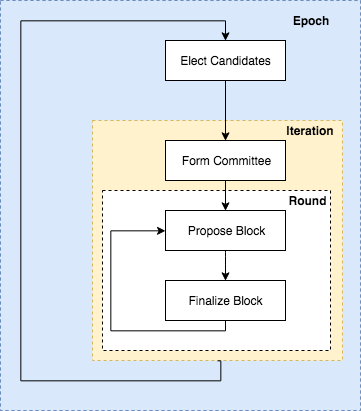
\includegraphics[width=0.5\textwidth]{Figura6}
	\label{fig:figure6}
	\caption{Randomized Delegated Proof of Stake (R-DPoS)}
\end{figure}

\subsubsection{Elezione dei candidati}
Tutti i nodi della rete IoTeX possono partecipare in questa fase votando per i candidati a partecipare commissione. Per incentivare i nodi a votare, il sistema assicura che i delegati condividano con i loro elettori le ricompense forgiate. I candidati formano un insieme di almeno 97 delegati; questo numero aumenterà in futuro per evitare ulteriormente la centralizzazione della potenza di mining. Una volta selezionati i candidati, questi saranno fissati per la durata di un'epoca, che consiste di 47 iterazioni.

\subsubsection{Formazione della commissione}
In ogni iterazione, viene selezionata una commissione di 11 elementi scelti a caso dal pool di candidati mediante VRF per la creazione dei blocchi nei successivi 11 round. L'idea è di usare l'hash del blocco dell'ultima iterazione e la chiave privata del nodo come input del VRF per produrre un output Booleano che indica se esso è stato selezionato come membro della commissione, una priorità che indica il suo livello per proporre un blocco, e una prova che indica i suoi requisiti per poter proporre il blocco in un certo round. L'uso di VRF è importante in quanto fornisce un modo non interattivo per ordinare tutti i delegati, per proporre blocchi in modo equo e in sicurezza. A tal fine, usiamo il VRF efficiente come quello utilizzato in Algorand \cite{c12}.

\subsubsection{Proposta del blocco}
In ogni round (che inizia all'incirca ogni 3 secondi), ogni nodo della commissione propone un nuovo blocco e lo trasmette alla rete, insieme con la priorità e la prova (forniti dal VRF). Solo il blocco proposto da un nodo della commissione con la priorità più alta e che non è stato già proposto nella stessa iterazione viene considerato dagli altri nodi, e viene chiamato blocco candidato.

\subsubsection{Finalizzazione del blocco}
Nello stesso round, tutti gli altri nodi utilizzano PBFT per votare a favore o contro il blocco candidato. Se più dei 2/3 dei nodi della commissione concordano sulla validità del blocco candidato, esso viene finalizzato ed aggiunto alla blockchain da tutti gli utenti della rete. Dopo di ciò, i passi \emph{proposta del blocco} e \emph{finalizzazione del blocco} vengono nuovamente eseguiti nel round successivo; se l'iterazione corrente è terminata, sarà formata un'altra commissione a caso, prima che \emph{proposta del blocco} e \emph{finalizzazione del blocco} vengano nuovamente eseguiti.

\subsection{Creazione di checkpoint periodici per i client leggeri}
Nelle reti IoT, ci aspettiamo che molti dispositivi siano dei client leggeri, ovvero quei nodi partecipanti della blockchain che non registrano la cronologia completa delle transazioni localmente. Considerando l'overhead di archiviazione della blockchain completa, ad es. oltre 100 GB per Bitcoin \cite{c4}, molti dispositivi embedded IoT a basso costo potrebbero non avere la capacità di scaricare la blockchain completa. Tuttavia, questi client leggeri hanno ancora la capacità di verificare rapidamente la correttezza della blockchain e di interagire con essa: l'idea è inclusa nel Whitepaper originale del Bitcoin di Satoshi \cite{c21}.
Tuttavia, l'utilizzo del PoS anziché del PoW ha uno svantaggio per i client leggeri. Quando si verifica la correttezza di una blockchain basata sul PoS, i client devono scaricare un elenco di chiavi pubbliche e firme per i proponenti di blocco e gli elettori, ed i gruppi di proponenti di blocco
e gli elettori possono cambiare per ogni singolo blocco. Quindi, quando i client leggeri tornano online dopo essere stati offline per un po', i client potrebbero aver bisogno di scaricare un gran numero di chiavi pubbliche e firme, e quindi verificarle tutte. Per mitigare questo problema di performance, Vitalik, l'inventore di Ethereum, ha proposto di creare dei checkpoint periodici sulla blockchain, chiamate \emph{epoche} \cite{c6}, ad esempio ogni 50 blocchi. Ogni checkpoint
può essere verificato basandosi sul checkpoint precedente, in modo tale che i client leggeri possano sincronizzarsi con l'intera blockchain molto più velocemente.

